% ============================================================================
% TEMPLATE PARA TRABAJOS PRÁCTICOS INDIVIDUALES (TPI)
% Asignatura: Ampliación de Bases de Datos
% Curso 2026/2027 - Universidad Loyola Andalucía
%
% TPI 3: Acceso a Bases de Datos: Arquitectura de Tres Niveles
% Estudiante: Fernando Martín González
% Profesor: Dr. Anier Soria Lorente
% Repositorio: https://github.com/fernandomartin04/spark-mercadona-ventas
% ============================================================================

\documentclass[a4paper,12pt]{article}

% ---------------------------------------------------------------------------
% Codificación, idioma y tipografía
% ---------------------------------------------------------------------------
\usepackage[utf8]{inputenc}
\usepackage[T1]{fontenc}
\usepackage[spanish,es-nodecimaldot]{babel}
\usepackage{lmodern}
\usepackage{microtype}
\usepackage{eurosym}

% ---------------------------------------------------------------------------
% Página y espaciado
% ---------------------------------------------------------------------------
\usepackage[a4paper,top=2.3cm,bottom=2.3cm,left=2.5cm,right=2.5cm]{geometry}
\usepackage{setspace}
\setstretch{1.12}
\setlength{\parindent}{0pt}
\setlength{\parskip}{0.5em}

% ---------------------------------------------------------------------------
% Colores e identidad visual (Universidad Loyola)
% ---------------------------------------------------------------------------
\usepackage{xcolor}
\definecolor{LoyolaBlue}{HTML}{082B66}
\definecolor{LoyolaCyan}{HTML}{5CC8DF}
\definecolor{SoftBlue}{HTML}{EEF5FA}
\definecolor{SoftGray}{HTML}{F5F6F7}
\definecolor{TextGray}{HTML}{374151}

% ---------------------------------------------------------------------------
% Imágenes, tablas y listas
% ---------------------------------------------------------------------------
\usepackage{graphicx}
\usepackage{booktabs}
\usepackage{array}
\usepackage{enumitem}
\usepackage{float}
\usepackage{caption}

% ---------------------------------------------------------------------------
% Código fuente
% ---------------------------------------------------------------------------
\usepackage{listings}
\lstdefinestyle{codigo}{
  basicstyle=\ttfamily\footnotesize,
  backgroundcolor=\color{SoftGray},
  frame=single,
  rulecolor=\color{LoyolaBlue!35},
  numbers=left,
  numberstyle=\tiny\color{TextGray},
  numbersep=6pt,
  breaklines=true,
  showstringspaces=false,
  tabsize=2,
  captionpos=b,
  keywordstyle=\color{LoyolaBlue}\bfseries,
  commentstyle=\color{green!45!black},
  stringstyle=\color{orange!60!black},
  literate={á}{{\'a}}1 {é}{{\'e}}1 {í}{{\'i}}1 {ó}{{\'o}}1 {ú}{{\'u}}1 {ñ}{{\~n}}1 {º}{{\textordmasculine}}1 {€}{{\euro{}}}1
}
\lstset{style=codigo}

% ---------------------------------------------------------------------------
% Matemáticas y enlaces
% ---------------------------------------------------------------------------
\usepackage{amsmath,amssymb}
\usepackage{url}
\usepackage[hidelinks]{hyperref}
\hypersetup{
  colorlinks=true,
  linkcolor=LoyolaBlue,
  urlcolor=LoyolaBlue,
  citecolor=LoyolaBlue,
  pdftitle={TPI 3 - Acceso a Bases de Datos y Arquitectura de Tres Niveles},
  pdfauthor={Fernando Martín González}
}

% ---------------------------------------------------------------------------
% Cabecera y pie de página
% ---------------------------------------------------------------------------
\usepackage{fancyhdr}
\usepackage{lastpage}
\pagestyle{fancy}
\fancyhf{}
\fancyhead[L]{\small\textcolor{LoyolaBlue}{Ampliación de Bases de Datos}}
\fancyhead[R]{\small\textcolor{TextGray}{TPI 3 - Arquitectura de Tres Niveles}}
\fancyfoot[L]{\small Universidad Loyola Andalucía}
\fancyfoot[R]{\small Página \thepage\ de \pageref{LastPage}}
\renewcommand{\headrulewidth}{0.6pt}
\renewcommand{\headrule}{\hbox to\headwidth{\color{LoyolaCyan}\leaders\hrule height \headrulewidth\hfill}}
\renewcommand{\footrulewidth}{0pt}

% ---------------------------------------------------------------------------
% Estilo de secciones
% ---------------------------------------------------------------------------
\usepackage{titlesec}
\titleformat{\section}{\large\bfseries\color{LoyolaBlue}}{\thesection.}{0.5em}{}
\titleformat{\subsection}{\normalsize\bfseries\color{LoyolaBlue}}{\thesubsection.}{0.5em}{}

% ---------------------------------------------------------------------------
% DATOS DEL TRABAJO
% ---------------------------------------------------------------------------
\newcommand{\TPINumero}{TPI 3}
\newcommand{\TPITitulo}{Arquitectura de Tres Niveles, Independencia de Datos y Acceso mediante ODBC, JDBC e Hibernate en Mercadona}
\newcommand{\Estudiante}{Fernando Martín González}
\newcommand{\FechaEntrega}{Noviembre de 2026}
\newcommand{\Profesor}{Dr. Anier Soria Lorente}
\newcommand{\RepoURL}{https://github.com/fernandomartin04/spark-mercadona-ventas}

\begin{document}

% ============================================================================
% PORTADA
% ============================================================================
\begin{titlepage}
  \thispagestyle{empty}
  \begin{center}
    
\includegraphics[width=0.65\textwidth]{logo_uloyola.png}

    \vspace{1.0cm}
    {\Large\bfseries\color{LoyolaBlue} Ampliación de Bases de Datos\par}
    \vspace{0.2cm}
    {\large Grado en Ingeniería del Software\par}
    {\large Curso académico 2026/2027\par}

    \vspace{1.2cm}
    \colorbox{SoftBlue}{%
      \parbox{0.88\textwidth}{%
        \centering
        \vspace{0.4cm}
        {\LARGE\bfseries\color{LoyolaBlue}\TPINumero\par}
        \vspace{0.3cm}
        {\large\bfseries\TPITitulo\par}
        \vspace{0.4cm}
      }%
    }

    \vfill
    \begin{tabular}{>{\bfseries}p{4.2cm} p{9.0cm}}
      Estudiante: & \Estudiante \\
      Profesor: & \Profesor \\
      Fecha de entrega: & \FechaEntrega \\
      Repositorio GitHub: & \footnotesize\url{\RepoURL} \\
    \end{tabular}

    \vfill
    {\small\color{TextGray} Universidad Loyola Andalucía}
  \end{center}
\end{titlepage}

% ============================================================================
% ÍNDICE
% ============================================================================
\tableofcontents
\newpage

% ============================================================================
% 1. PROBLEMA REAL Y CONTEXTO
% ============================================================================
\section{Problema real y contexto}

En el trabajo anterior (TPI 2) resolvimos la parte de análisis masivo de un supermercado como Mercadona en Sevilla, procesando 50.000 líneas de ticket con Spark SQL para guardar en PostgreSQL (\texttt{mercadona\_bi}) qué se recauda y cuál es el producto más vendido en cada tramo horario.

Sin embargo, cuando esa base de datos PostgreSQL pasa a usarse en el día a día de las tiendas por distintos empleados y programas, aparecen tres problemas prácticos muy claros:
\begin{enumerate}[leftmargin=1.0cm]
    \item \textbf{Diferentes perfiles ven cosas que no deben:} Un reponedor o cajero necesita saber qué producto se está agotando en cada hora y cuánto stock queda en el almacén, pero \textbf{no debe ver el coste de proveedor ni el margen de beneficio neto} que Mercadona le saca a cada producto (un dato confidencial que solo debe ver Dirección).
    \item \textbf{Cambios en las tablas que rompen los programas:} Si mañana añadimos una columna nueva al catálogo (por ejemplo, el pasillo donde se coloca el producto) o creamos un índice nuevo para acelerar las consultas, las aplicaciones de las tiendas no deberían dejar de funcionar.
    \item \textbf{Acceso seguro desde distintos lenguajes y herramientas:} Los scripts de consulta en Python, las aplicaciones de gestión en Java y los sistemas de actualización de stock necesitan conectarse a PostgreSQL usando estándares (\textbf{ODBC}, \textbf{JDBC} y un \textbf{ORM como Hibernate}) sin sufrir inyecciones SQL ni dejar pedidos a medias si algo falla.
\end{enumerate}

Por ello, en este TPI 3 ampliamos nuestro proyecto de Mercadona (manteniendo intacto todo el código previo de Spark y Python) para implementar la \textbf{arquitectura de tres niveles}, la \textbf{independencia física y lógica}, el acceso mediante \textbf{ODBC, JDBC e Hibernate} y las \textbf{buenas prácticas} del Tema 6. Todo el código actualizado se encuentra en el repositorio: \url{\RepoURL}.

% ============================================================================
% 2. NECESIDAD RELACIONADA CON LOS DATOS Y OBJETIVOS
% ============================================================================
\section{Necesidad relacionada con los datos y objetivos}

\subsection{Necesidad identificada}
Si las aplicaciones de los cajeros y las de los jefes de zona atacaran directamente las tablas base de PostgreSQL con el usuario administrador (\texttt{postgres}) y escribiendo consultas SQL concatenadas a mano, cualquier empleado tendría acceso a los costes confidenciales de los proveedores y cualquier cambio en la estructura de las tablas obligaría a reprogramar las aplicaciones.

\subsection{Objetivos del trabajo}
\begin{itemize}[leftmargin=1.0cm]
  \item Diseñar los tres niveles de abstracción (\textbf{interno, conceptual y externo}) sobre la base de datos \texttt{mercadona\_bi} en PostgreSQL, separando la vista del personal de tienda de la vista de dirección financiera.
  \item Comprobar en la práctica la \textbf{independencia física} (creación de índices B-Tree) y la \textbf{independencia lógica} (ampliación de columnas en las tablas conceptuales sin alterar las vistas externas).
  \item Conectar un cliente en Python mediante el estándar \textbf{ODBC} (\texttt{pyodbc}) usando un rol con privilegios mínimos (\texttt{empleado\_tienda}).
  \item Desarrollar una aplicación en Java que acceda a la misma base de datos tanto mediante \textbf{JDBC} (consultas parametrizadas y transacciones ACID) como mediante el ORM \textbf{Hibernate} (mapeo objeto-relacional de la entidad \texttt{ProductoCatalogo}).
\end{itemize}

% ============================================================================
% 3. CONCEPTOS DEL TEMA 6 APLICADOS
% ============================================================================
\section{Conceptos y tecnologías aplicadas (Tema 6)}

\subsection{Niveles de abstracción: interno, conceptual y externo}
Siguiendo la arquitectura ANSI/SPARC de tres niveles:
\begin{itemize}[leftmargin=1.0cm]
    \item \textbf{Nivel Conceptual:} Define la estructura lógica completa de la base de datos con sus tablas, tipos de datos y restricciones (\texttt{PRIMARY KEY}, \texttt{FOREIGN KEY} y \texttt{CHECK}). Sobre las tablas de tramos que ya teníamos del TPI 2, hemos añadido el catálogo maestro (\texttt{productos\_catalogo}, que incluye el dato sensible \texttt{coste\_proveedor}), la tabla de \texttt{tiendas} y la de \texttt{reposiciones\_stock}.
    \item \textbf{Nivel Interno:} Define cómo se almacenan y buscan físicamente los registros en disco. Hemos creado índices físicos B-Tree (\texttt{idx\_reposiciones\_tienda}, \texttt{idx\_productos\_categoria}) para que el motor de PostgreSQL localice los datos sin recorrer toda la tabla secuencialmente.
    \item \textbf{Nivel Externo:} Define las vistas parciales adaptadas a cada tipo de usuario:
    \begin{itemize}
        \item \texttt{vista\_personal\_tienda}: Cruza los productos más vendidos por hora con el catálogo mostrando precio de venta y stock, pero \textbf{ocultando el coste de proveedor}.
        \item \texttt{vista\_direccion\_mercadona}: Muestra el coste de proveedor, calcula el margen unitario (\texttt{precio\_venta - coste\_proveedor}) y obtiene el beneficio neto en euros por cada hora.
    \end{itemize}
\end{itemize}

\subsection{Independencia de datos: física y lógica}
\begin{itemize}[leftmargin=1.0cm]
    \item \textbf{Independencia física:} Capacidad de modificar el almacenamiento interno sin tocar el nivel conceptual. La aplicamos creando un nuevo índice físico (\texttt{idx\_reposiciones\_franja}) sobre la franja horaria sin que cambie ninguna tabla ni consulta.
    \item \textbf{Independencia lógica:} Capacidad de modificar el esquema conceptual sin romper el nivel externo ni los programas. La aplicamos añadiendo con \texttt{ALTER TABLE} una nueva columna (\texttt{pasillo\_ubicacion}) a \texttt{productos\_catalogo}; como las vistas externas solo seleccionan las columnas necesarias, las aplicaciones siguen funcionando igual sin tocar su código.
\end{itemize}

\subsection{Interfaces de acceso (ODBC y JDBC) y ORM (Hibernate)}
\begin{itemize}[leftmargin=1.0cm]
    \item \textbf{ODBC (\textit{Open Database Connectivity}):} Interfaz estándar a nivel de sistema operativo. Usamos el driver oficial \texttt{PostgreSQL Unicode} desde Python (\texttt{pyodbc}) para consultar la vista del personal de tienda.
    \item \textbf{JDBC (\textit{Java Database Connectivity}):} API estándar de Java para ejecutar sentencias SQL a bajo nivel mediante \texttt{Connection}, \texttt{PreparedStatement} y \texttt{ResultSet}.
    \item \textbf{ORM Hibernate:} Herramienta de mapeo objeto-relacional que traduce automáticamente filas de la tabla \texttt{productos\_catalogo} a objetos de la clase Java \texttt{ProductoCatalogo} (\texttt{@Entity}), evitando escribir sentencias \texttt{INSERT}, \texttt{UPDATE} o \texttt{SELECT} a mano.
\end{itemize}

\subsection{Buenas prácticas de desarrollo orientado a bases de datos}
\begin{enumerate}[leftmargin=1.0cm]
    \item \textbf{Principio de mínimo privilegio:} El rol \texttt{empleado\_tienda} solo tiene permiso \texttt{SELECT} sobre \texttt{vista\_personal\_tienda} y tiene revocado el acceso a \texttt{productos\_catalogo}.
    \item \textbf{Prevención de Inyección SQL:} Todas las consultas en ODBC, JDBC y HQL utilizan parámetros (\texttt{?} o \texttt{:cat}) en lugar de concatenar cadenas de texto.
    \item \textbf{Gestión de transacciones ACID:} Los pedidos de reposición se ejecutan con \texttt{setAutoCommit(false)}, confirmando con \texttt{commit()} o deshaciendo con \texttt{rollback()} ante cualquier fallo.
    \item \textbf{Cierre automático de recursos:} Uso de bloques \texttt{try-with-resources} en Java y \texttt{try/finally} en Python para no dejar conexiones abiertas colgadas.
\end{enumerate}

% ============================================================================
% 4. DESARROLLO DEL TRABAJO
% ============================================================================
\section{Desarrollo del trabajo}

\subsection{Implementación de los 3 niveles e independencia en SQL}
En el archivo \texttt{sql/02\_arquitectura\_3\_niveles.sql} hemos definido los tres niveles, los permisos del rol restringido y las pruebas de independencia física y lógica:

\begin{lstlisting}[language=SQL,caption={Extracto de \texttt{sql/02\_arquitectura\_3\_niveles.sql}: niveles, vistas, permisos e independencia}]
-- 1. NIVEL CONCEPTUAL: Catálogo con dato confidencial (coste_proveedor)
CREATE TABLE productos_catalogo (
    id_producto VARCHAR(20) PRIMARY KEY,
    nombre_producto VARCHAR(100) NOT NULL,
    categoria VARCHAR(40) NOT NULL,
    precio_venta NUMERIC(6,2) NOT NULL CHECK (precio_venta > 0),
    coste_proveedor NUMERIC(6,2) NOT NULL CHECK (coste_proveedor > 0),
    stock_actual INT NOT NULL CHECK (stock_actual >= 0)
);

-- 2. NIVEL INTERNO: Índices físicos B-Tree en disco
CREATE INDEX idx_reposiciones_tienda ON reposiciones_stock USING btree (id_tienda);
CREATE INDEX idx_productos_categoria ON productos_catalogo USING btree (categoria);

-- 3. NIVEL EXTERNO: Vista para empleados (sin coste_proveedor) y vista Dirección
CREATE VIEW vista_personal_tienda AS
SELECT pmv.franja_horaria, p.id_producto, p.nombre_producto, p.categoria,
       p.precio_venta, pmv.unidades_totales AS unidades_vendidas_tramo, p.stock_actual
FROM producto_mas_vendido_tramo pmv
JOIN productos_catalogo p ON pmv.id_producto = p.id_producto
WHERE pmv.tipo_ventana = '1_HORA' ORDER BY pmv.franja_horaria;

CREATE VIEW vista_direccion_mercadona AS
SELECT pmv.franja_horaria, p.id_producto, p.nombre_producto, pmv.unidades_totales,
       p.precio_venta, p.coste_proveedor,
       (p.precio_venta - p.coste_proveedor) AS margen_unitario_eur,
       ROUND((pmv.unidades_totales * (p.precio_venta - p.coste_proveedor))::numeric, 2) AS beneficio_neto_tramo_eur
FROM producto_mas_vendido_tramo pmv
JOIN productos_catalogo p ON pmv.id_producto = p.id_producto
WHERE pmv.tipo_ventana = '1_HORA' ORDER BY pmv.franja_horaria;

-- Mínimo privilegio: el empleado solo ve su vista externa
REVOKE ALL ON productos_catalogo FROM empleado_tienda;
GRANT SELECT ON vista_personal_tienda TO empleado_tienda;

-- 4. INDEPENDENCIA FÍSICA Y LÓGICA
CREATE INDEX idx_reposiciones_franja ON reposiciones_stock USING btree (franja_horaria);
ALTER TABLE productos_catalogo ADD COLUMN pasillo_ubicacion VARCHAR(30) DEFAULT 'Pasillo Central';
\end{lstlisting}

\subsection{Acceso mediante ODBC en Python (\texttt{04\_acceso\_odbc.py})}
El script \texttt{scripts/04\_acceso\_odbc.py} utiliza \texttt{pyodbc} y el driver \texttt{PostgreSQL Unicode} conectándose con el usuario restringido \texttt{empleado\_tienda}. Primero filtra de forma parametrizada (\texttt{?}) los tramos con al menos 900 unidades vendidas en \texttt{vista\_personal\_tienda}, y después intenta hacer un \texttt{SELECT} sobre \texttt{productos\_catalogo} para comprobar que PostgreSQL bloquea el acceso a los costes.

\subsection{Acceso mediante JDBC e Hibernate en Java (\texttt{java\_app/})}
Dentro de la carpeta \texttt{java\_app/} hemos creado la entidad ORM \texttt{ProductoCatalogo.java} mapeada con \texttt{@Entity} y \texttt{@Table(name="productos\_catalogo")}, y la clase principal \texttt{AppMercadona.java} que ejecuta ambas formas de acceso:

\begin{lstlisting}[language=Java,caption={Extracto de \texttt{AppMercadona.java}: JDBC con transacción ACID y ORM Hibernate}]
// PARTE 1: JDBC con try-with-resources, PreparedStatement (?) y Transacción ACID
try (Connection conn = DriverManager.getConnection(URL_JDBC, USUARIO, CLAVE)) {
    String sqlVista = "SELECT franja_horaria, nombre_producto, unidades_totales, "
                    + "precio_venta, coste_proveedor, beneficio_neto_tramo_eur "
                    + "FROM vista_direccion_mercadona WHERE beneficio_neto_tramo_eur >= ?";
    try (PreparedStatement ps = conn.prepareStatement(sqlVista)) {
        ps.setBigDecimal(1, new BigDecimal("500.00"));
        try (ResultSet rs = ps.executeQuery()) { /* Lectura de resultados */ }
    }

    // Transacción ACID para registrar un pedido de reposición en la tienda de Triana
    conn.setAutoCommit(false);
    String sqlInsert = "INSERT INTO reposiciones_stock (id_tienda, id_producto, unidades_reponer, franja_horaria) VALUES (?, ?, ?, ?)";
    try (PreparedStatement psInsert = conn.prepareStatement(sqlInsert)) {
        psInsert.setString(1, "MERC_SEV_TRIANA");
        psInsert.setString(2, "PROD_05");
        psInsert.setInt(3, 100);
        psInsert.setString(4, "12:00");
        psInsert.executeUpdate();
        conn.commit();
    } catch (Exception e) { conn.rollback(); }
}

// PARTE 2: ORM Hibernate trabajando directamente con objetos Java
try (SessionFactory factory = new Configuration().configure("hibernate.cfg.xml").buildSessionFactory();
     Session session = factory.openSession()) {
    // Cargamos la Cerveza Steinburg (PROD_05) como objeto Java sin escribir SQL
    ProductoCatalogo prod = session.get(ProductoCatalogo.class, "PROD_05");

    // Modificamos el stock en Java (+50 uds) y Hibernate genera el UPDATE solo
    Transaction tx = session.beginTransaction();
    prod.setStockActual(prod.getStockActual() + 50);
    tx.commit();
}
\end{lstlisting}

% ============================================================================
% 5. RESULTADOS OBTENIDOS
% ============================================================================
\section{Resultados obtenidos}

En la Figura~\ref{fig:odbc} se muestra la ejecución real del script \texttt{04\_acceso\_odbc.py}. Se observa cómo el driver ODBC devuelve correctamente los datos públicos de \texttt{vista\_personal\_tienda}, pero cuando el rol \texttt{empleado\_tienda} intenta leer la tabla base \texttt{productos\_catalogo} para ver el coste de proveedor, PostgreSQL deniega el permiso (\texttt{ERROR: permission denied for table productos\_catalogo}).

\begin{figure}[H]
  \centering
  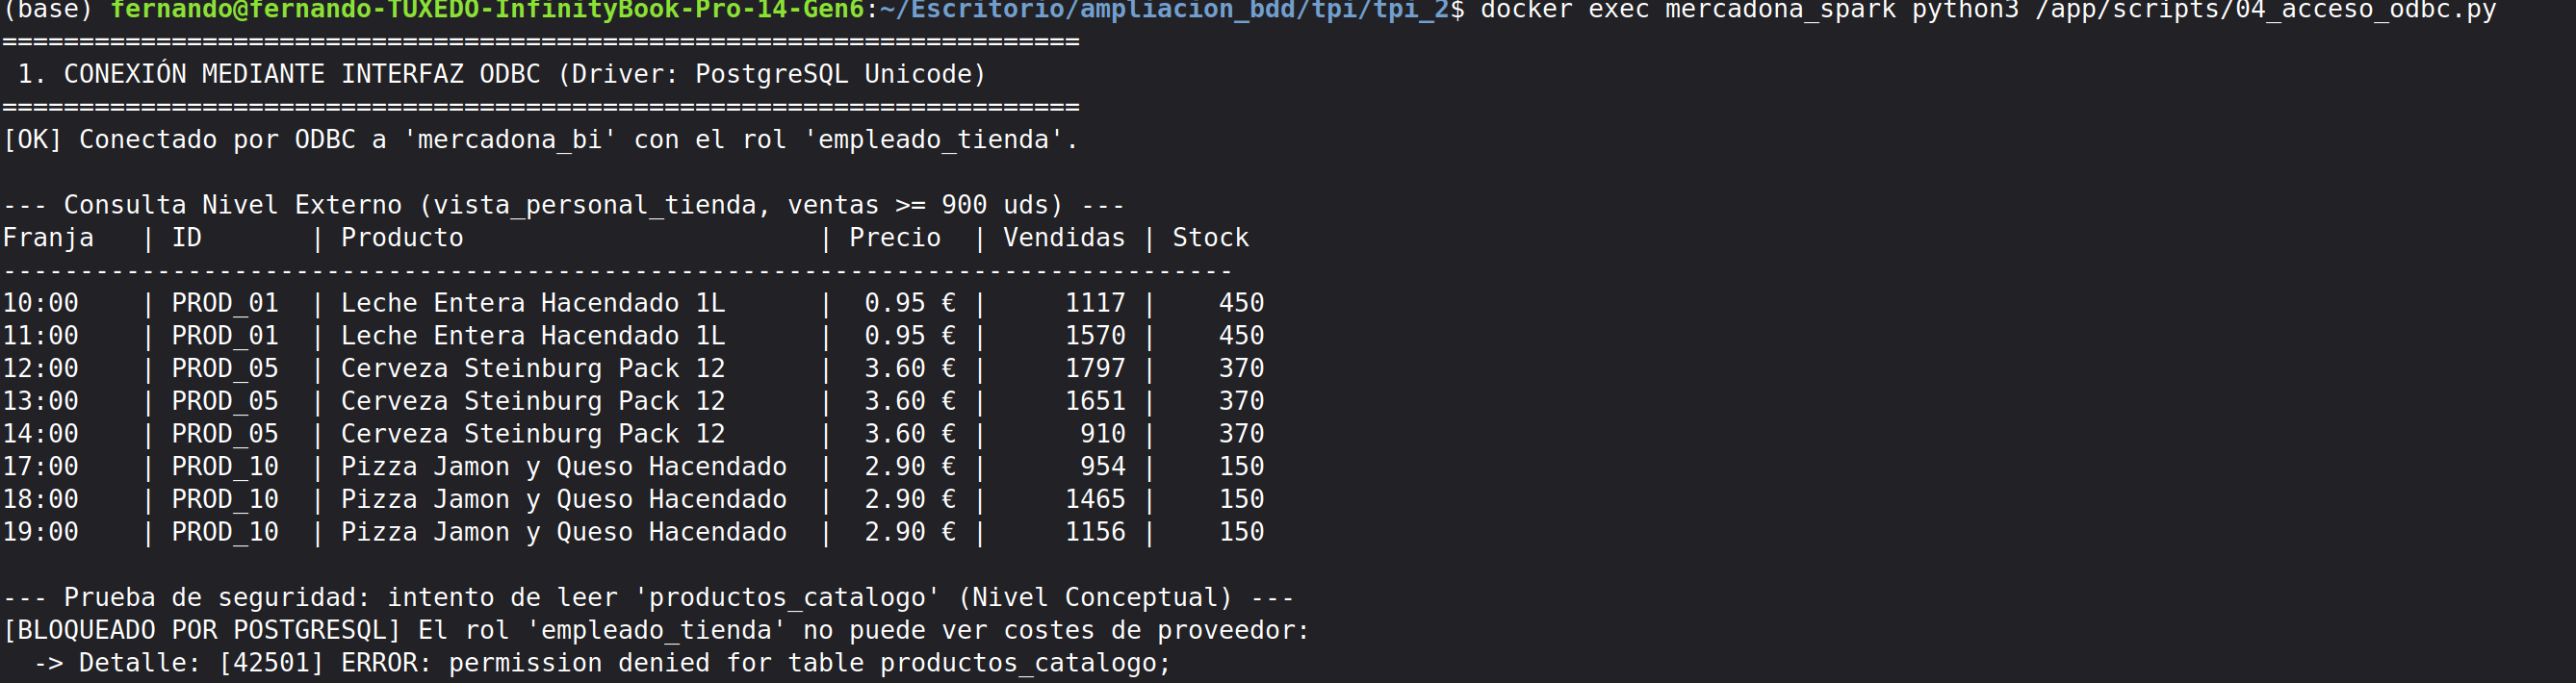
\includegraphics[width=0.92\textwidth]{imgs/captura_odbc.png}
  \caption{Ejecución del acceso por ODBC mostrando la consulta sobre la vista externa y el bloqueo de seguridad ante la tabla conceptual.}
  \label{fig:odbc}
\end{figure}

En la Figura~\ref{fig:jdbc_hibernate} se muestra la ejecución de la aplicación Java (\texttt{AppMercadona.java}). En la primera mitad, JDBC consulta la vista de Dirección obteniendo los tramos con beneficio neto superior a 500~\euro{} y confirma con \texttt{[COMMIT]} el pedido de reposición de 100 unidades en Triana. En la segunda mitad, Hibernate recupera el objeto \texttt{PROD\_05}, actualiza su stock de 320 a \textbf{370 unidades} generando automáticamente la sentencia \texttt{UPDATE}, y lista los productos lácteos mediante HQL.

\begin{figure}[H]
  \centering
  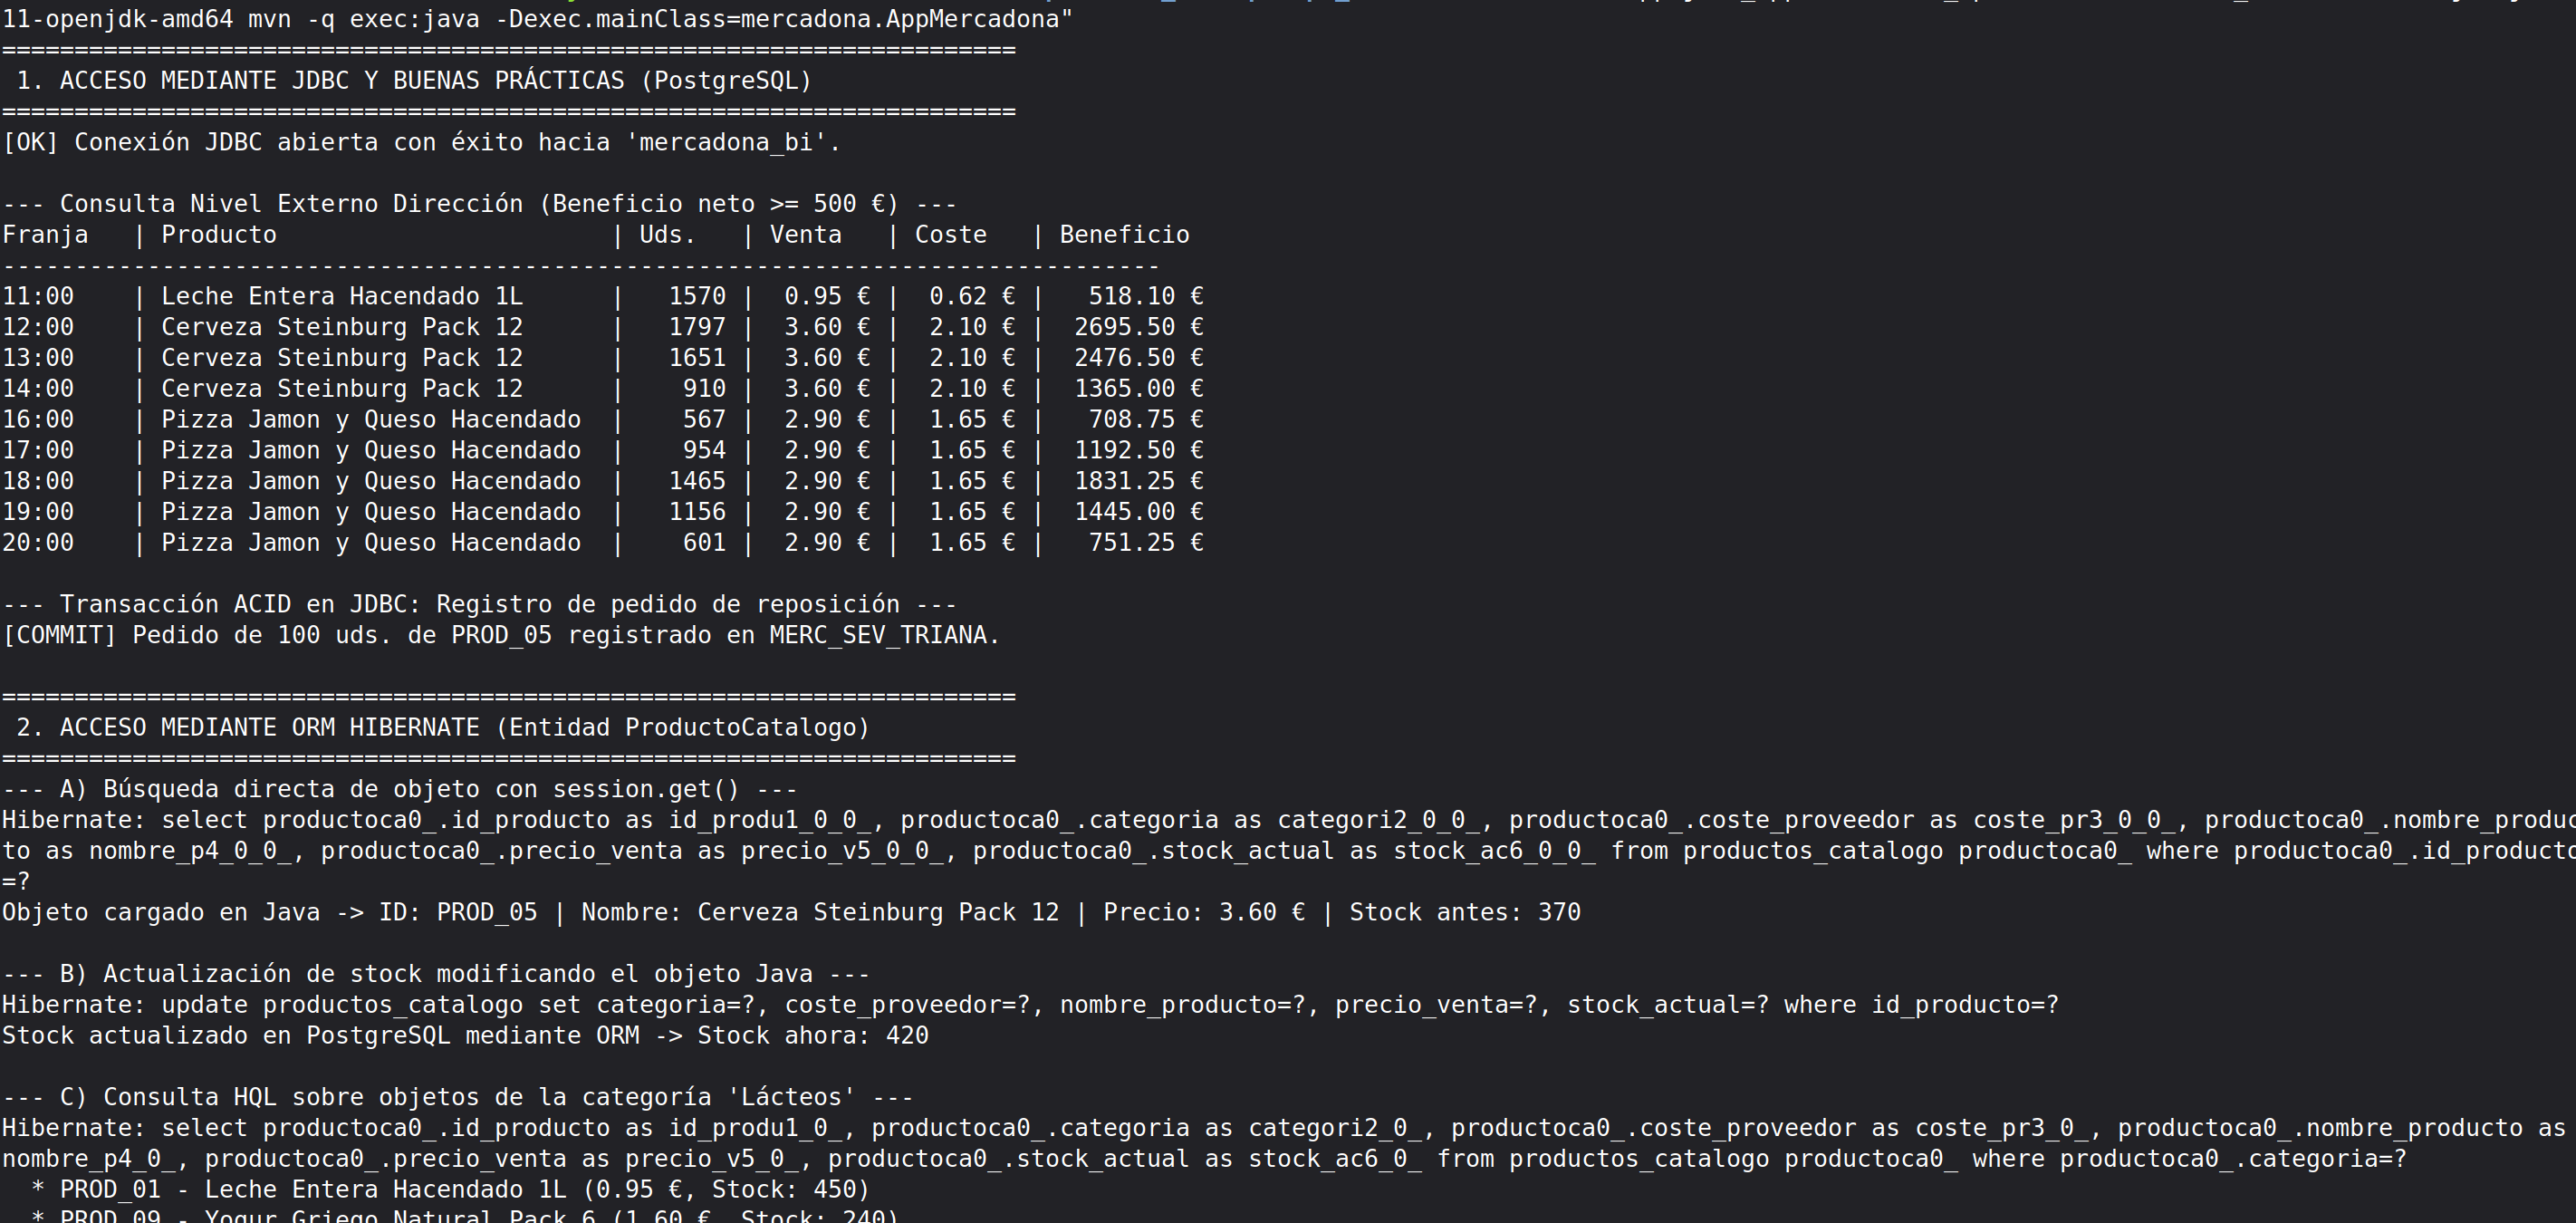
\includegraphics[width=0.92\textwidth]{imgs/captura_jdbc_hibernate.png}
  \caption{Ejecución en Java del acceso mediante JDBC (con transacción ACID) y mediante el ORM Hibernate.}
  \label{fig:jdbc_hibernate}
\end{figure}

Por último, en la Figura~\ref{fig:panel_tpi3} se muestra el visor web (\texttt{panel\_arquitectura\_tpi3.html}) generado por \texttt{05\_generar\_panel\_tpi3.py}, donde se comparan de un vistazo las dos vistas del nivel externo (con el stock ya actualizado a 370 por Hibernate y los costes ocultos en la vista de tienda) junto con la tabla de reposiciones actualizada por JDBC.

\begin{figure}[H]
  \centering
  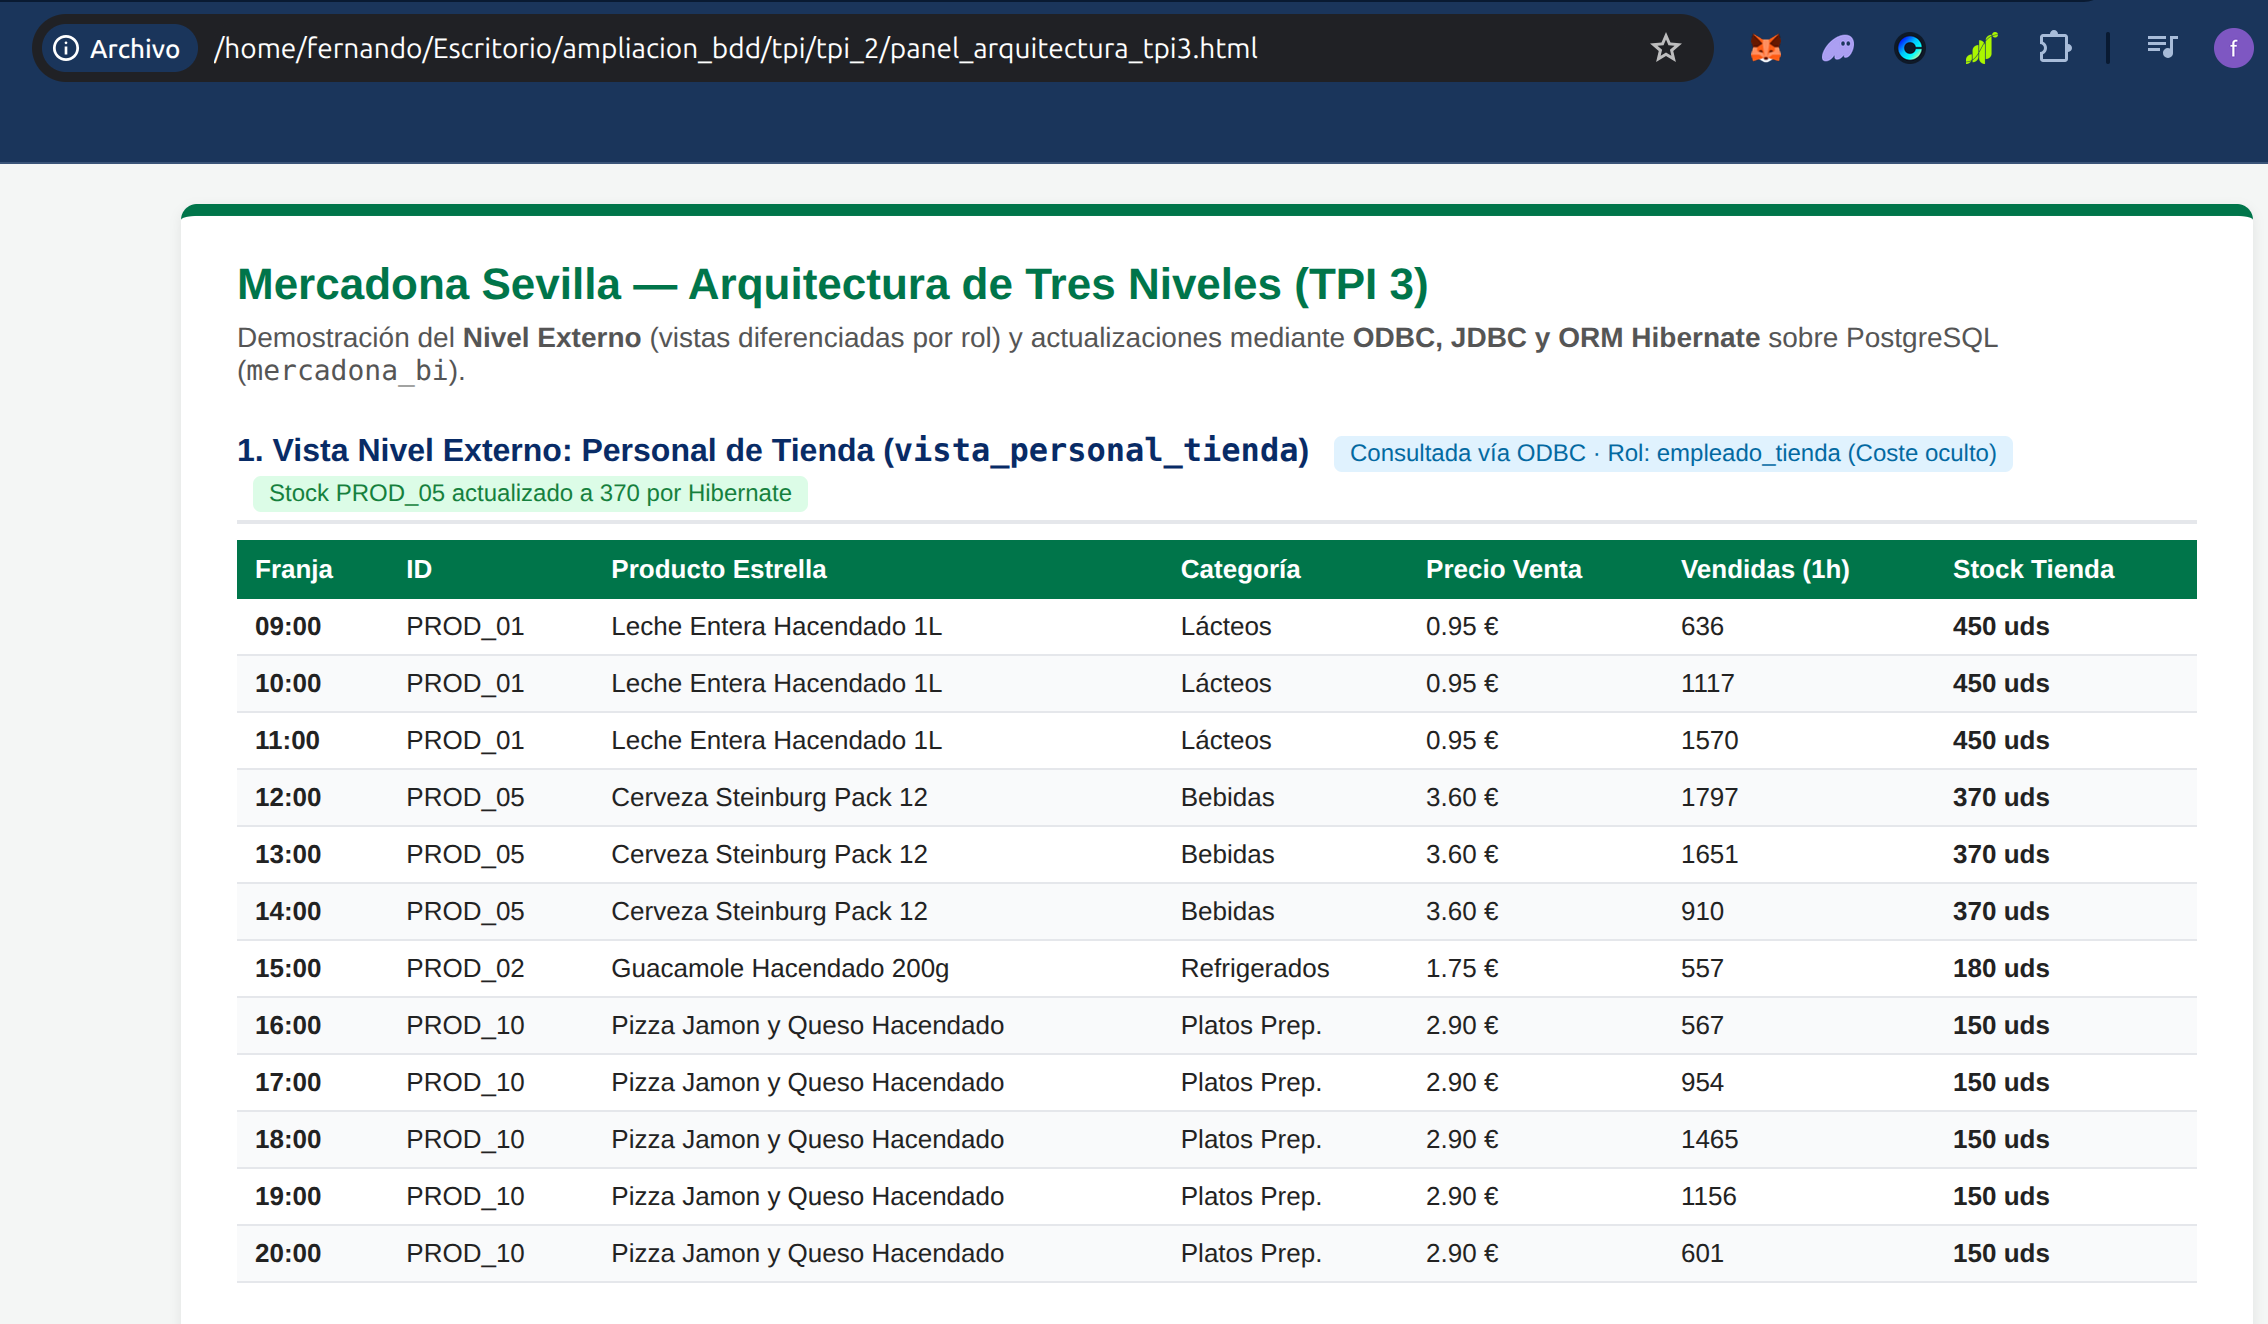
\includegraphics[width=0.90\textwidth]{imgs/captura_panel_tpi3.png}
  \caption{Visor HTML comparando las dos vistas del Nivel Externo y los cambios realizados por ODBC, JDBC e Hibernate.}
  \label{fig:panel_tpi3}
\end{figure}

% ============================================================================
% 6. ANÁLISIS E INTERPRETACIÓN DE LOS RESULTADOS
% ============================================================================
\section{Análisis e interpretación de los resultados}

\begin{enumerate}[leftmargin=1.0cm]
    \item \textbf{Protección real de datos confidenciales gracias al Nivel Externo:} En la vista de dirección vemos que en la franja de las 12:00 la \textit{Cerveza Steinburg Pack 12} tiene un coste de proveedor de 2,10~\euro{} frente a un precio de venta de 3,60~\euro{} (un margen de 1,50~\euro{}/pack que genera \textbf{2.695,50~\euro{} de beneficio neto} en una sola hora). Gracias a separar el nivel externo mediante vistas y permisos, el personal de tienda puede trabajar con los datos de ventas y stock desde ODBC sin ver en ningún momento esos márgenes comerciales.
    \item \textbf{Verificación de la independencia lógica:} Pese a haber alterado la tabla \texttt{productos\_catalogo} añadiendo la columna \texttt{pasillo\_ubicacion} en el nivel conceptual, ni el script ODBC en Python, ni la consulta JDBC, ni la entidad \texttt{ProductoCatalogo} de Hibernate se han roto, demostrando en la práctica para qué sirve desacoplar las capas.
    \item \textbf{Diferencia práctica entre JDBC e Hibernate:} Con JDBC tenemos control total sobre la consulta SQL (muy cómodo cuando queremos leer vistas con cálculos agregados como \texttt{vista\_direccion\_mercadona}), mientras que con Hibernate nos ahorramos escribir SQL para las operaciones CRUD sobre tablas de negocio: basta con hacer \texttt{prod.setStockActual(370)} en Java para que el ORM sincronice el cambio en PostgreSQL.
\end{enumerate}

% ============================================================================
% 7. DECISIONES TOMADAS Y JUSTIFICACIÓN
% ============================================================================
\section{Decisiones tomadas y justificación}

\begin{itemize}[leftmargin=1.0cm]
  \item \textbf{Continuar y ampliar el caso de Mercadona del TPI 2:} En lugar de crear un ejemplo aislado desde cero, hemos construido esta arquitectura directamente sobre la base de datos \texttt{mercadona\_bi} del TPI 2 sin modificar ni romper ninguno de los scripts anteriores de Spark SQL. Así el proyecto refleja cómo conviven en una empresa la parte analítica (Spark) y la parte operacional (3 niveles, ODBC, JDBC e Hibernate).
  \item \textbf{Combinar Python (ODBC) y Java (JDBC + Hibernate) en Docker:} Como ODBC se usa habitualmente desde scripts o herramientas externas y tanto JDBC como Hibernate son tecnologías nativas de Java, hemos integrado ambos dentro del mismo contenedor Docker para que todo se ejecute de forma reproducible sin ensuciar el sistema local.
  \item \textbf{Uso conjunto de JDBC e Hibernate según la tarea:} Hemos usado JDBC para consultar vistas de resumen e insertar un registro puntual con control manual de la transacción, e Hibernate para mapear la entidad principal del catálogo (\texttt{ProductoCatalogo}) donde resulta más natural trabajar con objetos Java.
\end{itemize}

% ============================================================================
% 8. CONCLUSIONES Y APRENDIZAJE
% ============================================================================
\section{Conclusiones y aprendizaje}

Este trabajo me ha permitido comprobar que la arquitectura de tres niveles (interno, conceptual y externo) no es solo teoría, sino un mecanismo muy práctico para que distintos perfiles de una empresa trabajen sobre la misma base de datos sin comprometer datos sensibles ni romper las aplicaciones cuando hay cambios en las tablas.

Asimismo, al programar sobre la misma base de datos PostgreSQL usando ODBC, JDBC e Hibernate he podido ver cuándo compensa cada tecnología y la importancia de aplicar siempre buenas prácticas básicas como parametrizar las consultas (\texttt{PreparedStatement}), usar transacciones ACID y cerrar las conexiones automáticamente.

% ============================================================================
% 9. DECLARACIÓN DE USO DE INTELIGENCIA ARTIFICIAL
% ============================================================================
\section{Declaración de uso de inteligencia artificial}

\textbf{Marque una opción y complete la información correspondiente:}

\begin{itemize}[label=$\square$,leftmargin=1.0cm]
  \item No he utilizado herramientas de inteligencia artificial en la realización de este trabajo.
  \item[\rlap{$\square$}{\raisebox{2pt}{\large\hspace{1pt}\textbf{X}}}] \textbf{Sí he utilizado herramientas de inteligencia artificial} como apoyo en este trabajo.
\end{itemize}

\textbf{Herramienta(s) utilizada(s):} \\
Google Gemini / Antigravity.

\textbf{Uso concreto realizado:} \\
Se utilizó como apoyo para repasar los conceptos del Tema 6, configurar los drivers de ODBC (\texttt{pyodbc}) y las dependencias de Maven para Hibernate en el contenedor Docker, estructurar el ejemplo de conexión en Java y asistir en el formato en LaTeX de la memoria siguiendo la plantilla oficial.

\textbf{Revisión y validación personal:} \\
La decisión de dar continuidad al caso práctico de Mercadona del TPI 2, el planteamiento de las vistas de tienda frente a dirección y la verificación de todos los scripts SQL, Python y Java se han realizado y probado personalmente en mi entorno local con Docker, asegurándome de comprender el funcionamiento completo para la defensa oral.

% ============================================================================
% 10. REFERENCIAS
% ============================================================================
\section{Referencias}

\begin{thebibliography}{9}

\bibitem{repo_github}
Fernando Martín González,
\textit{Proyecto Mercadona: Spark SQL, Arquitectura de Tres Niveles, ODBC, JDBC e Hibernate (Docker)},
Repositorio en GitHub, 2026.
\url{https://github.com/fernandomartin04/spark-mercadona-ventas}

\bibitem{hibernate_doc}
Red Hat / Hibernate Team,
\textit{Hibernate ORM 5.6 User Guide},
2024.
\url{https://docs.jboss.org/hibernate/orm/5.6/userguide/html_single/Hibernate_User_Guide.html}

\bibitem{postgres_jdbc_doc}
PostgreSQL Global Development Group,
\textit{PostgreSQL JDBC Driver Documentation},
2024.
\url{https://jdbc.postgresql.org/documentation/}

\bibitem{psqlodbc_doc}
PostgreSQL Global Development Group,
\textit{psqlODBC - PostgreSQL ODBC Driver},
2024.
\url{https://odbc.postgresql.org/}

\end{thebibliography}

\end{document}
